\documentclass[sigplan,screen]{acmart}

\usepackage{blindtext}
\usepackage{amsmath}
%\usepackage{amssymb}
\usepackage{xspace}
\usepackage{graphicx}
%\usepackage[texencoding=ascii]{biblatex}
\usepackage{tikz}
\usepackage{algorithm}
\usepackage{algpseudocode}
\usetikzlibrary{decorations.text}
\usetikzlibrary{arrows}

\tikzset{
    myarrow/.style={
        ->,
        >=angle 45 % change color as needed
    }
}

%\graphicspath{ {./} }
%\addbibresource{bibliography.bib}

%\usetikzlibrary{positioning}
%\usetikzlibrary{shapes}

%\newcommand{\relu}{\mathit{ReLU}}
%\newlength{\vnd}
%\newlength{\hnd}
%\newlength{\vds}
%\newcommand{\scl}{1}
%\tikzset{>=stealth}

%% Use the following for comments
\newcommand{\dmcmt}[1]{\textcolor{blue}{#1}}
\newcommand{\kmcmt}[1]{\textcolor{red}{#1}}
\newcommand{\sncmt}[1]{\textcolor{green}{#1}}

%% Use the following to disable comments
% \newcommand{\dmcmt}[1]{}
% \newcommand{\kmcmt}[1]{}
% \newcommand{\sncmt}[1]{}

\newcommand{\todo}[1]{\textcolor{orange}{TODO: #1}}
% \newcommand{\todo}[1]{}

%% Common stuff like ReLU
% TODO refactor to use this
\newcommand{\relu}{\textit{ReLU}\xspace}
\newcommand{\cnc}{$\mathcal{N}$\xspace}
\newcommand{\abs}{$\mathcal{N'}$\xspace}
\newcommand{\mcnc}{\mathcal{N}}
\newcommand{\mabs}{\mathcal{N'}}
\newcommand{\abcrown}{$\alpha,\beta-\mathit{CROWN}$ \cite{crown, autolirpa,
    convex-relax-barrier,alpha-crown-bab-fnc,beta-crown, bab-fw, gcp-crown,
    bab-nonlin} }
\newcommand{\marabou}{Marabou \cite{reluplex, marabou, marabouv2}}
\newcommand{\acasxu}{ACAS Xu \cite{acasxu, reluplex}\xspace}
\newcommand{\mnist}{VNNComp MNIST \cite{vnncomp-1-3, vnncomp-4, mnist}}
\newcommand{\pgd}{PGD-attack \todo{cite}}
\newcommand{\cegar}{CEGAR \cite{cegar-nn} \todo{cite}}
\newcommand{\dnn}{DNN\xspace}
\newcommand{\quality}{quality\xspace} % The word for measure of quality of abs
\newcommand{\inc}{\textit{inc}\xspace}
\newcommand{\dec}{\textit{dec}\xspace}
\newcommand{\posc}{\textit{pos}\xspace}
\newcommand{\negc}{\textit{neg}\xspace}
\newcommand{\cls}{\mathcal{C}}
\newcommand{\nr}[2]{n_{(#1,#2)}}
\newcommand{\vct}[1]{\boldsymbol{#1}}
\newcommand{\nrf}[2]{v_{(#1,#2)}}
\newcommand{\ob}[2]{o_{(#1,#2)}}
\newcommand{\hcluster}{hierarchial clustering \todo{cite}}
\newcommand{\gencex}{spurious input\xspace}

\renewcommand{\algorithmicrequire}{\textbf{Input:}}
\renewcommand{\algorithmicensure}{\textbf{Output:}}


\title{Unifying Syntactic and Semantic Abstractions for Deep Neural Networks}

\author{Sanaa Siddiqui}
%\authornote{}
\email{csy227516@iitd.ac.in}
%\orcid{}
\affiliation{
        \institution{IIT Delhi}
        \city{New Delhi}
        \country{India}
}
\author{Diganta Mukhopadhyay}
%\authornote{}
\email{diganta.m@tcs.com}
%\orcid{}
\affiliation{
        \institution{TCS Research}
        \city{Pune}
        \country{India}
}

\author{Mohammad Afzal}
\email{afzal.2@tcs.com}
\orcid{0000-0002-6173-3959}
\affiliation{
        \institution{TCS Research, Pune, India,}
        \city{and}
        \country{IIT Bombay, Mumbai, India}
}

\author{Hrishikesh Karmarkar}
\email{hrishi.karmarkar@tcs.com}
\orcid{0000-0002-9132-8356}
\affiliation{
        \institution{TCS Research}
        \city{Pune}
        \country{India}
}

\author{Kumar Madhukar}
\email{madhukar@cse.iitd.ac.in}
\orcid{0000-0001-5686-9758}
\affiliation{
        \institution{IIT Delhi}
        \city{New Delhi}
        \country{India}
}

\renewcommand{\shortauthors}{Sanaa et al.}

\begin{document}


\begin{abstract}
Deep Neural Networks (DNNs), today, are being trained and trusted for
performing fairly complex tasks, even in safety-critical applications such as
automated driving, medical diagnostics, and air-traffic control. Proving
trustworthiness, typically using formal verification or formal explainability,
is a difficult task though. The biggest challenge in this comes from the size
of the DNNs -- real-world networks are trained for performance, and
compromising size for accuracy is therefore a natural thing to do. To address
this issue, several abstraction methods have been proposed. This includes
techniques that perform an abstract analysis of the network, and those that
abstract or compress the network itself.  We study the latter, in which there
are two different approaches that have been taken: \emph{syntactic}
abstraction, with formal soundness guarantees, and \emph{semantic} abstraction
where the soundness guarantees are usually much weaker, and empirical. In this
paper, we propose to combine the semantic and syntactic approaches into a
single framework, to get the best of both worlds. This allows us to guide the
abstraction using global semantic information while still providing concrete
soundness guarantees based on syntactic constraints. Our experiments on
standard neural network benchmarks shows that this can be effective for both
verification as well as compression.
\end{abstract}

\iffalse

\begin{abstract}
Neural Networks are increasingly being used in several safety critical
applications, including medical imaging, self driving cars and aircraft
collision detection. To gain trust on the networks being deployed in safety
critical domains and reduce the risk of safety violations, several techniques
based on formal analysis has been proposed, including formal verification and
formal explainability. However, the scalability of these techniques is highly
sensitive to the size of the networks involved, limiting the applicability of
these techniques to real-world networks. To handle these scalability issues,
structural abstraction based on syntactic techniques have been proposed, and
while these provide formal soundness guarantees, they do not take into account
the semantic behavior of the network. On the other hand, neural network
compression and semantic abstraction \dmcmt{Jan, few lines in intro}
techniques take into account this information, but the soundness guarantees they
provide are generally much weaker, and empirical. We propose to combine both
the semantic and syntactic approaches into a single framework to try to obtain
the best of both worlds, guiding our abstraction using global semantic
information while still providing concrete soundness guarantees based on
syntactic constraints. We do this by constructing a partial order of best
possible merges using global semantic information, and represent it using a
tree-like data structure. Then we follow this tree to perform syntactic merge
and example guided \sncmt{Some other wording?} refinement operations. This
allows us to obtain abstract networks that is guided by global semantic
information while providing concrete soundness guarantees. We demonstrate the
effectiveness of these abstractions on standard neural network benchmarks via
experiments.
\end{abstract}

\fi


\maketitle

\section{Introduction}
\dmcmt{There may be repetation with abstract, but that is fine right?}

Advances in Deep Neural Networks (\dnn) have enabled the scalable solution of
several previously intractable problems such as image recognition and natural
language processing. Due to this, \dnn have increasingly assumed a central role
across various domains. These include several safety-critical domains like
healthcare \cite{b1}, where they contribute significantly to medical diagnosis
and predictive analysis \cite{b2}, and autonomous vehicles, where DNNs serve as
the backbone for sophisticated perception systems, supporting tasks such as
object recognition and decision making \cite{b3}. 

However, given the enormous size and the substantial resource requirements of these \dnn in terms of CPU, memory and power, their implementation on embedded devices and real-time systems is often infeasible. This issue becomes especially apparent when integrating DNNs into embedded and real-time systems for performing safety-critical tasks, such as obstacle recognition in autonomous vehicles. Furthermore, \dnn are well known to be vulnerable to adversarial~\cite{l-bfgs,fgsm,deep-fool,pgd,ground-truth-adv-attack,cw-attack}
and backdoor
attacks~\cite{backdoor-poisoning}, and are also difficult to interpret.
While a number of formal analysis techniques have been proposed to build
trust on the reliability of \dnn in safety-critical settings, including
verification \cite{reluplex,deeppoly,crown,beta-crown,cegar-nn}  and formal
explainability \cite{overview-fxai,minimal-image-fxai}, the size of the DNNs
\sncmt{Say here: and the NP-Hardness of solving queries involving DNNs}
continues to be the limiting factor for the scalability of these techniques.
To tackle both these issues, it is imperative to reduce the size of the \dnn
involved while maintaining a strong formal connection to the original network, and
preserving desirable safety properties.

%However, given the enormous size and the substantial resource requirements of
%these DNN solutions in terms of CPU, memory and power, their implementation
%on embedded devices is often infeasible.  This issue
%becomes especially apparent when integrating DNNs into embedded systems for
%performing safety-critical tasks, such as obstacle recognition in autonomous
%vehicles. 
%Additionally, \dnn are well known to be vulnerable to
%adversarial~\cite{l-bfgs,fgsm,deep-fool,pgd,ground-truth-adv-attack,cw-attack}
%and backdoor
%attacks~\cite{backdoor-poisoning}, and are also difficult to interpret.
%Therefore, to build trust on safety and business-critical embedded systems
%that utilize \dnn, it is critical to understand, interpret and validate their
%behaviour via formal analysis
%\cite{overview-fxai,minimal-image-fxai,backdoor-verification,nn-lander-verif,camera-verif-dsouza,generalization-verif}.
%While a number of techniques have been proposed to build
%trust on the reliability of \dnn in safety-critical settings, including
%verification \cite{reluplex,deeppoly,crown,beta-crown,cegar-nn}  and formal
%explainability \cite{overview-fxai,minimal-image-fxai}, the size of the DNNs
%continues to be the limiting factor for the scalability of these techniques.
%Therefore, for these two reasons, the applicability of \dnn in safety critical
% embedded systems remains limited.

A typical approach within formal methods to reduce the complexity of any object
while maintaining a strong formal connection with the original network is
\emph{abstraction}.
For \dnn, structural abstraction based on the \emph{syntax} (the local weights
and biases at each neuron of the DNN) forms the basis of several techniques
\cite{cegar-nn,cegarette,cleverest-nn,conv-abs-gk} 
that work by converting a large \emph{concrete}
DNN \cnc into a smaller \emph{abstract} DNN \abs via \emph{merging} groups
of neurons in \cnc into single neurons in \abs. 
Each such merge is done in a
way that ensures that there are \textit{concrete}, formal soundness guarantees
linking the behavior of \cnc and \abs, thus maintaining safety-critical
properties. 
In particular, one can verify properties on \abs, and
using the concrete soundness guarantees, lift the result to \cnc and argue
about its reliability. 
However, while these techniques have been shown to extend the scalability of
neural network verification techniques, they do not take the \emph{semantic}
behavior of the network into account, thereby producing sub-optimally large
\abs. \cite{cegar-nn}. 
In fact, in \cite{cegar-nn}, the \abs produced was sometimes observed to be
larger than the original \cnc.
This sub-optimality with respect to size prevents these techniques from being
useful for compressing \dnn for deployment in safety-critical
resource-constrained environments.

On the other hand, neural network compression techniques \cite{dnn-compression}
and semantic abstraction techniques \cite{deep-abstract,lin-comb-abs-jan} take
into account the global \textit{semantic} behavior of the network, and are able
to achieve a significant reduction in size.
However, heuristic based compression techniques \cite{dnn-compression} do not
formally maintain any connection with \cnc, while semantic abstraction
\cite{deep-abstract,lin-comb-abs-jan} techniques only provide some limited
kinds of formal connections with \cnc. 
In particular, the guarantees provided by clustering based methods like
\cite{deep-abstract} are limited to lifting specific bound propagation based
proofs from \abs to \cnc, 
and those provided by linear combination based methods like
\cite{lin-comb-abs-jan} only bound the difference in behavior of \abs and \cnc
on a finite subset of the input space.
Thus, without strong formal guarantees connecting the behaviors of \abs and
\cnc, the \abs may not preserve desired safety properties.

%Structural abstraction based on the \textit{syntax} (the local weights and
%biases at each neuron of the DNN) forms the basis of several techniques
%attempting to alleviate this issue
%\cite{cegar-nn,cegarette,cleverest-nn,conv-abs-gk}. 
%These techniques work by converting a large \textit{concrete}
%DNN \cnc into a smaller \textit{abstract} DNN \abs via \textit{merging} groups
%of neurons in \cnc into single neurons in \abs. 
%Each such merge is done in a
%way that ensures that there are \textit{concrete}, formal soundness guarantees
%linking the behavior of \cnc and \abs. 
%Then, one can make queries on \abs, and
%using the concrete soundness guarantees, lift the result to \cnc and argue
%about its reliability. 
%However, these techniques do not take into account the
%global \textit{semantic} behavior of the network, thus produce potentially
%suboptimal abstractions.

%On the other hand, neural network compression techniques \cite{dnn-compression}
%and semantic abstraction techniques \cite{deep-abstract,lin-comb-abs-jan} take
%into account the global \textit{semantic} information within the network.
%However, compression techniques provide no soundness guarantees, while 
%semantic abstraction techniques provide limited soundness guarantees. In
%particular, the guarantees provided by clustering based methods like
%\cite{deep-abstract} are limited to
%lifting specific bound propagation based proofs, and those provided by
%linear combination based methods like \cite{lin-comb-abs-jan} only characterize
%soundness on a finite subset of the
%input space. This limits the applicability of these techniques to situations
%where concrete, hard guarantees may be necessary.

\dmcmt{In this section, we end up saying "setting up a cegar loop thrice"}

In this work we combine the syntactic and semantic approaches into a single
framework for generating an abstract network. By splitting and labeling the
neurons \textit{inc} and \textit{dec}, similar to \cite{cegar-nn}, and
restricting ourselves to merges involving only similarly labeled neurons, we
provide a concrete formal link the behavior of \cnc and \abs via
syntactic constraints. At the same time, to take into account the global
semantic behavior, we introduce a semantic closeness metric between two neurons
in the same layer. Using this metric, we construct a tree of merge operations
that captures the relative contribution of each merge to the quality of the
abstraction. We propose a refinement procedure \dmcmt{here implicitly we say we
are setting up cegar loop} that uses
this tree as a guide
to undo the merge operations that contribute most to the poor quality of \abs.
We show that in the resulting refined network, groups of neurons that remain
merged are semantically closer than neurons that get un-merged. Thus, we are
able to refine \abs in a way that is optimal with respect to the semantic
behavior. Thus, combining both syntactic and semantic approaches, our framework
is able to find an \abs that preserves desired safety properties and is of a
smaller size.

We assemble these pieces into an abstraction-refinement framework \dmcmt{ here
again we say set up cegar loop} that can
generate a small size \abs by starting with a fully merged network and
iteratively refining until a strong enough network is obtained. To demonstrate
the usefulness of this framework we set up a
\cegar loop\dmcmt{ here again we say set up cegar loop}  
to verify the \acasxu networks. In these experiments we find that we
are able to produce smaller networks than existing works that are still strong
enough to verify the property.

\dmcmt{Alternate para, without the repeats::}

In this work we combine the syntactic and semantic approaches into a single
framework for generating an abstract network. By splitting and labeling the
neurons \textit{inc} and \textit{dec}, similar to \cite{cegar-nn}, and
restricting ourselves to merges involving only similarly labeled neurons, we
provide a concrete formal link the behavior of \cnc and \abs via
syntactic constraints. At the same time, to take into account the global
semantic behavior, we introduce a semantic closeness metric between two neurons
in the same layer. Using this metric, we construct a tree of merge operations
that captures the relative contribution of each merge to the quality of the
abstraction. We propose a CEGAR framework where
the refinement procedure
uses this tree as a guide
to undo the merge operations that contribute most to the poor quality of \abs.
In the resulting refined network, groups of neurons that remain
merged are semantically closer than neurons that get un-merged, 
Thus, combining both syntactic and semantic approaches, our framework
is able to find an \abs that preserves desired safety properties and is of a
smaller size.

To demonstrate
the usefulness of this framework we set up 
experiments
verifying the \acasxu networks. In these experiments we find that we
are able to produce smaller networks than existing works that are still strong
enough to verify the property.


\todo{ Change 'node' to 'neuron' wherever applicable}
\section{Background}
\subsection{Neural Network}
\dmcmt{There was some general definitions of what an nn is in this section,
removed for now, nor really necessary, maybe can add a notation section if at
all necessary}
\newline
\sncmt{Notation is important. Will be required in the upcoming sections.}
\newline
We conceptualize neural networks as directed acyclic graphs 
comprising three types of layers: the input layer, intermediate hidden layers, 
and the output layer. Our goal is to focus on the abstracting feed forward networks, 
where neuron values are computed based on preceding layer neuron values. 
Neurons in our network are denoted as $n_{(i,j)}$, where `$i$' signifies the 
neuron number in layer `$j$'. The weight matrix between layers `${j-1}$' and `$j$' 
is denoted as `$W_{{j-1}, j}$', and the bias matrix for layer `$i$' is denoted as 
`$B_{i}$'. The value of the `$i^{th}$' neuron in layer `$j$' for a given input vector 
is represented by `$v_{(i,j)}$', and `$V_{j}$' encompasses all such `$v_{(i,j)}$' values for layer 
`$j$'. The function $o_{(i, j)}$ takes a list of input vectors and outputs a list of
corresponding `$v_{(i,j)}$' for a particular neuron $n_{(i, j)}$. 

The computation of `$V_{j}$' involves applying an ``activation function ($\phi$)" 
to the ``weighted sum":

\[V_{j} = \phi(W_{{j-1}, j} \cdot V_{j-1} + B_{j}).\] 

We confine our activation function to the Rectified Linear Unit (ReLU), 
which can be expressed as $V_{j} = \max(W_{j-1, j} \cdot V_{j-1} + B_{j}, 0)$.

\subsection{ Formal Analysis of Neural Networks }
\label{s:form-an}
\dmcmt{This section used to be titled Neural Network Verification, and explained
    the general idea of neural net verif, and some stuff on prop encoding. We
    are not doing exclusively verif. So, some more general and shorter
    discussion on formal analysis of nn added.}

Several techniques and methods have been studied to improve the reliability and
trustworthiness of \dnn deployed in safety critical settings via formal
analysis. This includes verifying \dnn with respect to a given
safety property \cite{reluplex, cegar-nn, deeppoly, cegarette, cleverest-nn,
conv-abs-gk, deep-abstract, lin-comb-abs-jan}, providing formal explanations of
the behavior of the \dnn \cite{minimal-image-fxai, overview-fxai}, and others.
\dmcmt{Is the and others okay? Ref the backdoor attacks work?} To provide the
formal guarantees behind the analysis performed, all of these techniques rely on
making \textit{neural network queries}. 

These neural network queries are of the form $(P, \mcnc, Q)$, and ask if
for all inputs $x$ to $\mcnc$ for which the formula $P$ holds
the formula $Q$ also holds on the output $\mcnc(x)$. While there are several
tools that can handle such queries, like \marabou and \abcrown, scalability
remains an issue, and so reducing the size of \cnc is desirable.

\subsection{Semantic Compressions and Abstractions with Empirical Guarantees}
\label{s:emp-abs}
\dmcmt{What is a better word than 'weak' here? Does 'empirical' work here?}

Several techniques utilise semantic information, typically extracted via
simulation of the \dnn, to obtain \abs. \dmcmt{Say: to improve scalability? }.
Neural network compression techniques \todo{cite}, produce small \abs, but the
behavior of \abs in connection to \cnc is only characterized empirically.
Similarly, some semantic abstraction techniques \cite{lin-comb-abs-jan} provide
bi-simulation guarantees bounding the difference in the behavior of \abs and
\cnc on a finite set of input points, typically a subset of the training
dataset. Since these techniques characterize the behavior of \abs only on a
finite set of
input points, the trust obtained on the connection between \cnc and \abs is only
of a empirical nature.
Other techniques like \cite{deep-abstract} use bi-simulation to lift
interval bound propagation performed on \abs to get sound bounds on \cnc. While
this does provide a sound proof, interval bounds are typically not strong enough
to prove many interesting and practically relevant neural network queries.
\todo{cite}

\subsection{Concrete Guarantees on Neural Network Abstractions}
\label{s:conc-abs}
\kmcmt{We need to add one is good for analysis and one is good for proofs.
Not in negative light.} \dmcmt{ Even for analysis, we are trying to claim that
our concrete guarantees are better than the empirical ones right? We show a case
of proof, and a case of compression, so things are clear right?}

The notion of providing concrete guarantees on the behavior of \abs relative to
\cnc has been formalized in \cite{cegar-nn}. In particular, guarantees of the
form $\forall x, \mabs(x) \geq \mcnc(x)$ \dmcmt{
Should I format this as definition?} are useful as a general notion of concrete
guarantees in many settings. Two such settings are as follows: 

Firstly, since any general neural network query can be converted to a query of
the form $(P, \mcnc, y < c)$ for some $c$ \cite{cegar-nn, reluplex} \todo{See
\cite{cegar-nn}, they have another citation for this encoding} \dmcmt{It seems
that \cite{cegar-nn}, \cite{reluplex} and we have 3 different encodings, but
generally based on the same idea of implementing bool combs via extra nn
layers}, such a guarantee is
useful for dispatching the query on a smaller network \cite{cegar-nn, cegarette,
cleverest-nn}. This immediately makes an \abs with these guarantees useful for
accelerating several formal analysis techniques (Section \ref{s:form-an}).

Furthermore, such guarantees are also useful for safe compression of \dnn.
Consider the case of medical diagnosis\todo{cite} or aircraft
collisions\cite{acasxu}, where
for safety reasons, a classifier should be biased towards not producing false
negatives. Guarantees such as above can formally ensure that the compressed \abs
never produces any more false negatives than \cnc. \todo{Ref next sections}.
\dmcmt{Should this be here?}

Therefore, in this work we focus on developing a framework\dmcmt{Is this word
here okay?} that produces
abstract networks with this guarantee.

\subsection{Quality of Abstractions and Spurious Points}
\label{s:qual}

A generally useful notion with respect to abstraction is \textit{quality},
which we as the number of \textit{spurious inputs} that witness a difference in
the relevant behavior of \abs and \cnc. In the context of using \abs to
accelerate formal analysis of \dnn, these spurious inputs may simply be
\textit{spurious counterexamples} \cite{cegar-nn, cleverst-nn} to a query
involving \abs that are not counterexamples for the same query involving \cnc.
This notion may be generalized to other uses of abstractions as well. For
instance, for safe compressions, they may be inputs from a dataset which
are falsely classified as positive by \abs. \todo{Ref section}

\subsection{Syntactic Neural Network Splitting and Merging}
\label{s:nn-sam}

\dmcmt{Given that this section is critical to understanding our soundness
    guarantees, and that this is mostly existing work, how much space should be
spent here? Can we trust reader to read \cite{cegar-nn}}

\dmcmt{Start a running example here}

To transform \cnc into \abs so that the soundness guarantees hold, we follow
\cite{cegar-nn} to \textit{split} neurons in \cnc into copies labelled with
labels from \{\inc, \dec\} $\times$ \{\posc, \negc\} so that any
increase (decrease) in the value of a neuron labelled
\inc (\dec) only leads to an increase in output value. Then,
following \cite{cegar-nn}, a sound abstraction can be obtained by
\textit{merging} all similarly labelled neurons as follows: if the neurons have
the label \inc (\dec), replace incoming edges from the same
previous layer neuron with a single edge with the maximum (minimum) of the
original edge weights. Outgoing edges to the same next layer neuron are replaced
with a single edge with the sum of the weights for both the \inc and \dec case.

\dmcmt{Do we need to add a reference for 2-class? It may help shorten section.} 

We make a slight modification to the above: as a first optimization step, we
re-merge the two copies of the \abs neurons that are otherwise the same, but
have \posc and \negc labels respectively. This can always be done without
changing the behavior of the network since these copies will have the same \inc,
\dec labels and the same incoming weights. \dmcmt{Is this clear? Is it better to
write this as a lemma, and then put a proof in appendix?} This optimisation
allows us to discard the \posc and \negc class information, and reduces the size
of the maximally merged network.

Note that this process only considers the syntactic structure of the network, no
semantic information is used.

\subsection{ Syntactic Refinement }
\dmcmt{Jan Kretinsky's abstraction is based on semantic info, refinement is not.
Given this, do we really need to talk about Jan's refinement here? If yes,
how to weave it in?}

The fully merged network obtained in Section \ref{s:nn-sam} may not have
sufficient quality (Section \ref{s:qual}) to be useful. For instance, when doing
formal analysis, there may be too many spurious counterexamples. In such
situations, a common approach to obtain a better quality \abs is to perform
refinement steps based on a spurious counterexample $x$ \cite{cegar-nn,
cegarette, cleverest-nn}. \dmcmt{While \cite{cegar-nn} does it only for spurious cexes,
it can be directly extended to spurious inputs. But, I'm speaking in terms of
sp cex here to avoid confusion. Should I say spurious input instead?} In
existing techniques this is typically done restoring a single neuron in \cnc
that had been merged \abs. The neuron chosen is typically one whose contribution
to $x$ is estimated to be the highest.

These techniques, however, do not consider any semantic behavior to guide their
refinement. As such, the refinement process tends to produce a large number of
restored neurons identical to neurons in \cnc, leading to and \abs of large
size, while retaining a single abstract neuron formed by merging a large group
of neurons in \cnc, affecting the quality of \abs.  \todo{example}

\section{Methodology}
\dmcmt{
    In same example, we immediately arrive at a better picture. 
    This picture is equivalent to refining and merging back in the Elboher's
setting.}

\dmcmt{ This general part of the paper has this duty: bridge the gap from
whatever gk is doing, that it creates poor quality abstractions with a lot of
singleton neurons, ---> our tree. Answer the question: why and where did the
tree come from. Motivate the tree}

\dmcmt{Two ways of doing this.}

\dmcmt{\textbf{Way 1}: There is a PO (PO1) of all possible merges. GK is
    exploring very small part of it - leads to bad quality, singletons, etc.
    Exploring all of it is hard. But, using semantic info, we can restrict
    ourselves to a smaller part of it, we don't need to explore all of PO1.
    Because, if semantic info tells us that it is better to merge ab than ac,
    then we can discard the entire part of PO1 where ac has been merged. Once
    this cut has been done, we get a tree.
}

\dmcmt{\textbf{Way 2:} GK's ref doesn't produce good quality, and we want a
    better abstraction/refinement by bringing in semantic info. What does
    semantic info give? IO similarity of groups of neurons in \cnc. This gives a
    ordering between possible merge operations, which actually forms a tree.
    Then, each \abs correspond to certain cuts in the tree.
}

\dmcmt{\textbf{Current Decision:} Do way 2, but have 1-2 lines referencing the
    idea in way 1 that says that by following the semantic information we avoid
    exploring all possible \abs
}

\dmcmt{Madhukar supports this. Refiment in our case should be based on priority
    between two merges using semantic info. This priority adds an extra
    dimension. Describe things strictly from the perspective of doing a full
    abstraction then prioritise refinement, don't mix the other perspective of
doing a prioritised abstraction.}

\dmcmt{Get a semantic closeness factor, between pairs of merge groups. Similar
    idea to GK's sameness of color. This gives a natural way to construct a tree
     /PO, and go from there.}

Our methodology involves two broad steps:
\begin{enumerate}
    \item Finding a tree structure that represents the order in which neurons should be merged.
    \item Using that structure to guide a CEGAR approach in order to help reduce
        number of refinement steps. \dmcmt{We can't really claim this in any
            way.. but we can claim that we search through a space with higher
        quality \abs, guided by global semantic information.}
\end{enumerate} 

\subsection{Tree and Merges:}

To establish the merging order of neurons, we create a tree structure wherein leaf nodes represent the original neurons, and non-leaf nodes represent merge groups. The construction of the tree follows a bottom-up approach, prioritizing the merging of similar neurons and delaying the merging of dissimilar ones. Similarity is ascertained through observation vectors. Consider simulating the network with distinct input values and observing the fluctuating values of a particular neuron corresponding to those inputs. The collection of these observed values constitutes an observation vector. 

\begin{figure}[H]
    \centering
    \includegraphics[width=0.5\textwidth]{diagrams/tree_merges.pdf}
    \includegraphics[ width=0.47\textwidth]{diagrams/Order_of_Merge.pdf}
    \caption{Order Of Merging}
    \label{Figure: Order Of Merging}
\end{figure}


In Figure \ref{Figure: Order Of Merging}, when we input values \{1, 2, 3\} to the neuron $n_0^{0}$ at different time instances, we obtain corresponding values \{1.5, 3, 4.5\}, forming the observation vector at neuron $(n_1^{1},Inc)$. For instance, considering three neurons $n_i^{w}$, $n_j^{w}$, and $n_k^{w}$ with observation vectors $\mathcal{\nu}(n_i^{w})$, $\mathcal{\nu}(n_j^{w})$, and $\mathcal{\nu}(n_k^{w})$, the merging sequence adheres to the following conditions: 

If $||\mathcal{\nu}(n_i^{w}) - \nu(n_j^{w})||_{2} \leq ||\nu(n_i^{w}) - \nu(n_k^{w})||_{2}$ and $||\nu(n_i^{w}) - \nu(n_j^{w})||_2 \leq ||\nu(n_j^{w}) - \nu(n_k^{w})||_{2}$, then $n_i^{w}$ and $n_j^{w}$ are initially merged into a representative neuron $\alpha$, followed by the merging of $\alpha$ and $n_k$. Here $||\nu(n_i^{w}) - \nu(n_j^{w})||_{2}$ computes the ``$\textit{Euclidean  Distance}$" between the observation vectors $\nu(n_i^{w})$ and  $\nu(n_j^{w})$.


In Figure \ref{Figure: Order Of Merging}, for the first layer, the initial merge would involve the neuron $(n_0^{1},Inc)$ with $(n_1^{1},Inc)$, forming $\textit{Merge 1}$, then we would combine $(n_2^{1},Inc)$ and $(n_3^{1},Inc)$, forming $\textit{Merge 2}$. Finally we combine $\textit{Merge 1}$ and $\textit{Merge 2}$ into the root node. 

As we progress up the tree, the degree of over-approximation rises. This is due to the increasing difference between observation vectors as we ascend. Therefore, the sub-trees closer to the root are indicative of coarser merges, whereas the ones farther from the root represent finer merges. 



\subsection{Using Counter-Examples to make cuts in the Tree} 
We are guided by this tree as a prospective refinement method. Starting with the entire tree where everything is merged. When the solver detects a spurious counterexample `$\beta$', we leverage it to refine the network. This process commences by identifying the ``culprit neuron $\gamma$'' selected for refinement. A ``culprit neuron'' in a merge group is selected on the basis of how much the neuron contributed to the output. If change in output of  neuron changes the value of the output neuron significantly then that neuron is a good candidate for ``culprit neuron". 

Following this, we reverse all merges dependent on the culprit neuron $\gamma$. Therefore, refinement essentially involves finding a cut-point in the tree, precisely where all merges dependent on the culprit neuron $\gamma$ are undone. Each cut produces a set of trees, the merge groups then consist of neurons in the leaf nodes of the  these trees. Therefore finding new merge groups for refinement is therefore just finding a cuts in the tree.

\begin{figure}
    \centering
    \includegraphics[width = 0.5\textwidth]{diagrams/before_and_after_cut_2.pdf}
    \caption{Trees and Cuts}
    \label{Figure 2}
\end{figure}

Consider Figure \ref{Figure 2}, illustrating the merging sequence of neurons $(n_0^{1}, Inc)$, $(n_1^{1}, Inc)$, $(n_2^{1}, Inc)$, and $(n_3^{1}, Inc)$. If, for instance, the neuron $(n_3^{1}, Inc)$ is identified as the problematic neuron based on a counter-example, we will reverse all the merges dependent on the $(n_3^{1}, Inc)$ neuron, including $\textit{Merge 2}$ and the $\textit{Root Node}$ merge. Consequently, after implementing this reversal indicated in Figure \ref{Figure 2}, our refinement phase will yield three distinct merge groups. The first merge group comprises two neurons, namely $(n_0^1, Inc)$ and $(n_1^1, Inc)$. The second merge group and the third merge have single neurons $(n_2^1, Inc)$ and $(n_3^1, Inc)$, respectively.

\subsection{Culprit Neurons} 

A neuron, denoted as $\gamma$, is designated as a culprit neuron within a
specific layer when absolute value of the product of the difference between
$(v_{Rep(\gamma)}$ and $v_{\gamma})$ and the effective weight is maximized.
\todo{Add the 3 different methods generating counter-examples. Scores should be
avg over $\beta$ for a particular $\gamma$.}

$||(v_{Rep(\gamma)} - v_{\gamma})||_{2} \cdot |(\textit{effective\_weight})|$

In this context, $Rep$ signifies the representative neuron for neuron $\gamma$, $v_{\gamma}$ represents the value of the neuron $\gamma$ at counter-example $\beta$ and $\textit{effective\_weight}$ represents the how much does the value of output neuron changes with respect to change in the value of the neuron under consideration, essentially corresponding to the ``$\textit{gradient}$'' at that particular counter-example ``$\beta$''.

\begin{algorithm}
    \caption{Finding Cuts in the Tree (find\_new\_merge\_groups)}
    \begin{algorithmic}[1]
        \State $\gamma= \arg \max_i \|v_{Rep(i)} -v_i \|_2 \cdot | \textit{effective\_weight}| $ 
        \State Find a sequence of nodes, $t_1,t_2,t_3,..,t_k$ representing a  path from $t_1=$root to $t_k=\gamma$.
        \State Remove the nodes $t_1,t_2,..,t_{k-1}$ denoting the merges dependent on $\gamma$ through this path, leading to our connected tree being split into a collection of disconnected sub-trees.
        \State New merge groups are the leaf nodes in our disconnected graph.
    \end{algorithmic}
    \hspace*{\algorithmicindent} \textbf{Output} New Merge Groups
\end{algorithm}

\subsection{Optimality of the Trees}
Our objective is to determine the most efficient order for merging neurons, minimizing the introduction of over-approximation at each step. This approach aims to avoid creating networks with excessive over-approximation, which could lead to the generation of spurious counter-examples in response to queries. Opting not to mitigate over-approximation at each step would result in an increased number of refinement steps. This essentially entails making additional solver calls, incurring significant costs to eliminate the spurious counter-examples.


Nevertheless, during the initial merging process (until saturation is reached), the root node ``$\rho$'' will exhibit the same level of over-approximation across all conceivable merging scenarios—for all possible tree sequences. Nevertheless, when we descend one level down the tree to explore the children nodes of our original root node $\rho$ for the purpose of identifying a cut for refinement, we discover varying levels of over-approximation manifesting in the root nodes of the resultant sub-trees. These differences are a result of the different merging scenarios pursued to construct those individual trees.

\begin{algorithm}[H]
\caption{Cluster Merging Algorithm (find\_abstraction\_tree)}
\label{Cluster Merging Algorithm}
\begin{algorithmic}[1]
    \State Initialize every simulated distance vector as a singleton cluster.
    \State Initialize $C=\{v_1,v_2,v_3,..\}$ as the set of singleton clusters.
    \State Initialize a Binary Tree $T$ with leaves as $\{(n_1),(n_2),(n_3),..\}$ corresponding to $\{v_1,v_2,v_3,..\}$.
    \State Initialize $V$ as a set of visited nodes, empty at first.
    
    \Function{MergeFunction}{$u, v$}
        \If{All nodes are classified as \textbf{Inc}}
        {
        
            \Return $\max(u, v)$
        }
        \Else{ }
        {
        
            \Return $\min(u, v)$
        }
        \EndIf
    \EndFunction
    
    \While{$|C|>1$}
        \State $v_j, v_j = \arg\min_{\substack{a, b \in C}} \| a - b \|_2$
        \State Set $w=\text{MergeFunction}(v_i,v_j)$
        \State Let nodes from $T$ not in $V$ corresponding to $v_i,v_j$ be $m_i$ and $m_j$
        \State Remove $v_i,v_j$ from $C$ and add $w$ to $C$.
        \State Make $(m_i \cup m_j)$ the parent of $(m_i)$ and $(m_j)$ in tree $T$
        \State Add $m_i$ and $m_j$ to $V$.
    \EndWhile
\end{algorithmic}
\end{algorithm}

While the optimal tree, representing the optimal merging sequence, can aid in the refinement process by guiding the reversal of merges, finding such an optimal tree poses is extremely challenging. Even when dealing with only `n' Increment (Inc) neurons that have been merged to saturation, the total number of possible trees is given by $(2n-3)!!$, making the task of determining the truly optimal tree from these options extremely challenging.

Since finding this ideal tree is a challenging task, we employ hierarchical clustering (Algorithm \ref{Cluster Merging Algorithm}) as an approach to approximate and derive such a tree. Initially, we simulate our network using a set of `$k$' inputs. Subsequently, we employ cluster analysis on these `$k$' points to construct a hierarchical arrangement of clusters. This process initiates with data points corresponding to simulated values (observation values in the observation vector) of a neuron  forming their own cluster. The clusters are then systematically combined based on their similarity, thereby generating a hierarchy of clusters. The choice of similarity measure is the ``$distance \hspace{1mm} metric$" between clusters. We have used ``$Euclidean \hspace{1mm} Distance$" as our distance metric. Given that the data points to perform this hierarchical clustering originate from the values of the simulated neurons, this hierarchical clustering effectively reflects the methodology we employ to merge the neurons.

For example, in Figure \ref{Figure: Order Of Merging}, we conducted a simulation of our network on three data points. Subsequently, we examined the observation vectors corresponding to these points. Utilizing the hierarchical clustering algorithm, the initial selection for merging  will involve $(n_0^{1}, Inc)$ and $(n_1^{1}, Inc)$ because of the fact that their Euclidean distance is minimum. This forms $\textit{Merge 1}$ in Figure \ref{Figure: Order Of Merging}. The observation vector for $\textit{Merge 1}$ ($\nu_\textit{Merge1 }$) is the max of the $\nu((n_0^{1}, Inc))$ and $\nu((n_1^{1},Inc))$ which is \{1.5, 3, 4.5\}. For decrement nodes the observation vector would be minimum of the observation vector of the corresponding decrement nodes. The next merging step involved selecting $\nu((n_2^{1}, Inc))$ and $\nu((n_3^{1}, Inc))$ and merging these two neurons, representing $\textit{Merge 2}$ in Figure \ref{Figure: Order Of Merging}. The observation vector for $\textit{Merge 2}$ is now \{4, 8, 12\}. Ultimately, the Merge1 merge group is merged with the $\textit{Merge 2}$ merge group to create the Root Node in our network.

\begin{figure}[H]
    \centering
    \includegraphics[width = 0.5\textwidth]{diagrams/good_vs_bad_merges.pdf}
    \caption{Ways of Merging}
    \label{Figure 3}
\end{figure}

This approach of merging neurons based on similarity proves advantageous as it helps in reducing number of refinement steps. For instance, consider the task of checking whether $\forall v_{0}^{0} \in [0, 1]$ implies $v_{0}^{2} < 10$. If we had the neuron $(n_{3}^{1}, Inc)$ as the culprit neuron and then if we follow the second merging approach depicted in Figure \ref{Figure 3}, then we would have been compelled to reverse both $\textit{Merge 1}$ and $\textit{Merge 2}$. However, by employing the first merging approach, undoing only the $\textit{Merge 2}$ becomes sufficient, resulting in a reduction in the number of refinement steps required.


\subsection{Overall Algorithm}
\begin{algorithm}[H]
    \caption{Overall Algorithm}
    \label{Overall Algorithm}
    \begin{algorithmic}[1]
        \State $\mathcal{N'}$ = split\_Inc\_Dec($\mathcal{N}$)
        \State $\mathcal{N''}$ = abstract\_network($\mathcal{N'}$)
        \State simulation\_dict = simulate\_network($\mathcal{N'}$)
        \State $\mathcal{T}$ = find\_abstraction\_tree($\mathcal{N'}$, $simulation\_dict$)
        \If{verify($\mathcal{N''}$, $\kappa$, $\lambda$) is UNSAT}{

            \Return Property Holds
            }
        \Else
            \State Extract counter-example $\beta$
            \If{$\beta$ is not a spurious counter-example}
            {

                \Return ($\beta$, Property Violated)
            }
            \Else
                \State Find culprit neuron $\gamma$
                \State $merge\_groups$ = find\_new\_merge\_groups($\mathcal{T, \gamma}$)
                \State $\mathcal{N''} = get\_abstract\_network(merge\_groups)$
                \State \textbf{goto} step 5
            \EndIf
        \EndIf
    \end{algorithmic}
\end{algorithm}

\section{Experiments} 

We have implemented our method in python\footnote{The entirety of the code,
networks, datasets, and properties utilized in our evaluation will be made
available via a publicly hosted code repository in the camera ready version.}, 
utilizing the NumPy library for linear algebra
operations and the SciPy library for an implementation of \hcluster.
We have used a linkage-matrix based data structure similar to the one used in
SciPy to store the tree, and have precomputed and cached several
operations that may need to be repeated every refinement iteration. This allows
us to quickly perform the merge and split operations and calculate the
scores (Section \ref{s:refinement}), without having to do (relatively)
expensive tree traversal operations in each iteration of the abstraction
refinement loop. 

Using this implementation, we have performed a set of experiments demonstrating
the effectiveness of our abstraction technique for verification of neural
network queries on the \acasxu set of networks, using both the original safety
properties from \cite{reluplex} and the $\epsilon$-robustness properties
introduced in \cite{cegar-nn}. To do so, we set up a \cegar loop (Section
\ref{s:abs-ref-fw}) using our abstraction technique, using the \neuralsat solver
as the underlying solver to dispatch the verification queries on \abs.
We compare our abstraction framework with the existing \cegar framework proposed
in \cite{cegar-nn} \footnote{We have used a faithful re-implementation of this
framework that follows exactly the procedure in the paper, with the only two
distinctions being that we are using a two-class classification as seen in
\cite{chauhan2022efficiently,liu2022abstraction,10.1145/3644387},
and that the call to verify the \abs obtained in each iteration is sent to an
instance of the \neuralsat solver as opposed to \marabou. } 
setting a 
timeout of 200 seconds for each instance in the benchmark and for both the
our technique and the existing work.
The experiments were run on a machine running on Intel(R) Core(TM) 
i7-6700 CPU with 8 CPUs running at 3.40GHz, having 16 GB RAM and running running 
Ubuntu 22.04 LTS.

If the \abs produced has multiple neurons with the exact same set of incoming
edges in the same layer, these neurons compute the same function and are
redundant. Therefore, as an added optimization step, we safely \textit{re-merge}
them by taking the sum of the outgoing edges. Note that this does not change the
behavior of \abs.

%to
%demonstrate the usefulness of our technique. To begin with, we demonstrate 
%the application of our method within a CEGAR loop, as outlined in \cite{cegar-nn}, 
%for verifying the \acasxu properties (refer to Section \ref{s:acas-verif}). 
%In these experiments, we employed \neuralsat as the solver in the backend.
%In our subsequent experiments, we illustrate the utility of our abstraction 
%technique in achieving efficient compression of \dnn within safety-critical 
%environments. We ensure that this compression doesn't introduce any new 
%false negative classifications, as detailed in Section \ref{s:exp-mnist-comp}. 
%This necessity is crucial, especially in scenarios such as medical diagnosis 
%and collision detection, where the application of \dnn as classifiers necessitates 
%precise measures to prevent false negative classifications for specific classes.
%Finally, we demonstrate how our technique may be used to obtain abstract 
%networks with the aim of proving a given property, plotting the number of 
%spurious counterexamples introduced as the size of the abstract network 
%reduces (Section \ref{s:exp-mnist-rob}). 

%If the \abs produced has multiple neurons with the exact same set of incoming
%edges in the same layer, these neurons compute the same function and are
%redundant. Therefore, as an added optimization step, we safely \textit{re-merge}
%them by taking the sum of the outgoing edges. Note that this does not change the
%behavior of \abs.

%The experimental results in Tables \ref{t:acas-verif}, \ref{t:acas-verif-robustness} and Figure
%\ref{f:scatter-netsizes} were produced on a machine running on Intel(R) Core(TM) 
%i7-6700 CPU with 8 CPUs running at 3.40GHz, having 16 GB RAM and running running 
%Ubuntu 22.04 LTS. The results in Tables \ref{t:mnist-compr-summary}, \ref{t:acas-ncex}
%and Figures \ref{f:mnist-class}, \ref{f:acas-ncex-samples} were run on a 
%machine running on an Intel(R) Core(TM) i7-9700K with 8 CPUs running at
%3.60GHz, having 16 GB RAM and running Ubuntu 22.04 LTS. 
%The results in Figures \ref{f:mnist-prop-samples} and Table \ref{t:mnist-prop-summary} were produced on a 
%machine running on an Intel(R) Core(TM) i7-13700 with 24 CPUs running at
%5.20GHz, having 32 GB RAM and running Ubuntu 23.10.

%\subsection{Verification of \acasxu}
%\label{s:acas-verif}

%In this set of experiments, we demonstrate the effectiveness of our abstraction
%technique for verification of neural network queries on the \acasxu set of
%benchmarks. To do so, we set up a \cegar loop (Section \ref{s:abs-ref-fw}) using
%our abstraction technique, where on each \abs generated we call \neuralsat. 
%If the solver returns a spurious counterexample, we use
%that as $\vct{\beta}$ to refine our network according to Section
%\ref{s:refinement}.  

%For these experiments, we have used \neuralsat as the solver. 
%We compare our abstraction framework with an existing \cegar framework proposed
%in \cite{cegar-nn} \footnote{We have used a faithful re-implementation of this framework that
%follows exactly the procedure in the paper, with the only distinction being that
%the call to verify the \abs obtained in each iteration is sent to an instance of
%the \neuralsat solver as opposed to \marabou. \dmcmt{Is this okay?}}. We set a
%timeout of 200 seconds for each instance in the benchmark and for both the
%our technique and the existing work \cite{cegar-nn}.

\begin{table}
    \centering
        \begin{tabular}{ |c|c|c|c|c| }
        \hline
        Method                   & No. Safe    & No. Unsafe & No. Timeout & Average Size \\ 
        \hline
        Ours                     &   121       & 43         & 16          &  335.3\\
        Existing \cite{cegar-nn} &   118       & 43         & 19          &  536.0\\
        \hline                                                                
        \end{tabular}
        \caption{Summary of \acasxu on original safety properties }
        \label{t:acas-verif}
    \vspace{-1cm}
\end{table}
\begin{table}
    \centering
    \begin{tabular}{ |c|c|c| }
    \hline
    Method                   & Percentage Verified  & Average Size \\ 
    \hline
    Ours                     &   100\%              &  27.9\\
    Existing \cite{cegar-nn} &   100\%              &  31.5\\
    \hline                                                                
    \end{tabular}
    \caption{Summary of \acasxu on robustness properties }
    \label{t:acas-verif-robustness}
    %\vspace{-1cm}
\end{table}


Tables \ref{t:acas-verif} and \label{t:acas-verif-robustness} summarizes the
results on these benchmarks. We
find that using our framework, we are able to perform better than the existing
\cegar approach \cite{cegar-nn} on the original safety properties, verifying
more networks to be safe, while we do not loose performance on the robustness
properties. 

\begin{wrapfigure}{r}{0.5\textwidth}
    \vspace*{-1cm}
    \includegraphics[scale=0.2]{figs/scatter-cegar-our-nerualsat.png}
    \caption{Scatter plot of network sizes produced by our framework vs existing
    work \cite{cegar-nn}}
    \label{f:scatter-netsizes}
    \vspace*{-1cm}
\end{wrapfigure}

For each framework, we collected the final \abs at the end of the \cegar
iterations, for which either the property can be proved to be safe, or 
the solver is able to find an actual counterexample, or the solver times out.  
Figure \ref{f:scatter-netsizes} shows a scatter plot comparing the sizes of these final \abs
obtained by our framework and by existing work \cite{cegar-nn} for each instance
in the benchmark. The average sizes of these \abs over all instances are
reported in the `Average Size' columns in tables \ref{t:acas-verif} and
\label{t:acas-verif-robustness}. 

It is apparent from the Figure \ref{f:scatter-netsizes}, 
table \ref{t:acas-verif} and table \ref{t:acas-verif-robustness} that compared 
to the existing techniques, we are explore smaller \abs that are effective 
at proving or disproving the property in question.
This shows that using semantic information to guide the \cegar process can
effectively find more efficient abstractions than the existing technique.

Note that in our experiments, we found that the time taken by both our \cegar
approach and the existing \cegar approach \cite{cegar-nn} was more than what the
\neuralsat solver takes for the \acasxu benchmarks. However, while we would
expect the solver call times to exponentially scale with network size, the
overheads from the abstraction procedure will not scale exponentially. Thus, for
larger and larger benchmarks, being able to find smaller \abs will produce a
significant difference in times. Furthermore, we believe that a verified \abs is
useful beyond verifying a single property - it may be used for other related
queries, or may be useful as a safely deployable compressed network.

Additionally, we find that the final solver times on the \abs are actually
comparable with the times obtained on the original un-abstracted \cnc. In
general it has may observed, both by our experiments and in \cite{cegar-nn},
that the effort needed to verify a network is dependent
on more than just network size. In fact, in \cite{cegar-nn},
they are able to achieve smaller solver times on larger networks. 
While it is true that in general the worst-case performance of neural network
solvers will almost certainly remain exponential in the size of the network
\cite{reluplex}, other factors on which the performance of neural network
solvers may depend on remains an interesting direction of future work. 


\section{Related Work}

In response to the increasing use of neural networks in safety-critical settings, 
various techniques have been developed to analyze their behavior, including 
verification, explainability, etc. 

Our work closely relates to the syntactic structural abstraction technique that
proposes to reduce the network size by merging similar
neurons \cite{cegar-nn,cegarette,cleverest-nn}, and employs a
counterexample-guided refinement. They have used
syntactic constraints to achieve concrete soundness guarantees. But unlike our
approach, their work does not take into account the global \textit{semantic}
behavior of the network, thus producing potentially suboptimal abstractions.
At the same time, the approach proposed in \cite{deep-abstract} performs a
semantic analysis to decrease the network size, but it leads to an
\emph{approximation} instead of an abstraction. The approximation allows
lifting certain bound propagation based proofs, but not the concrete gurantee
that one gets from~\cite{cegar-nn}. Also, in \cite{lin-comb-abs-jan} the
authors have used linear combinations of neurons to compress the networks, but
their method only provides guarantees on a finite dataset. In comparison, we
provide concrete soundness guarantees that allows us to lift any proofs from
the abstract network back to the original network.

In general, methodologies for verifying neural networks generally fall into two
main categories: sound and complete methods
\cite{reluplex,formal-ver-piece-wise,comp-reachability-analysis,comp-milp,comp-out-range,comp-max-resilience,marabou,comp-safety-ver-dnn,beta-crown,alpha-crown-bab-fnc,gcp-crown},
and sound and incomplete methods
\cite{deeppoly,crown,incomp-dual-approach,incomp-abs-inp,incomp-robustness-certi,incomp-boost-robustness}.
Sound and complete methods aim to explore the entire state space to verify the
properties of neural networks.
In contrast, sound and incomplete methods employ an overapproximation
of the state space, sacrificing completeness for 
scalability and efficiency.

An instance of a sound and complete methodology is Reluplex, which extends the 
simplex algorithm \cite{simplex} to 
handle ReLU constraints. Initially, it focuses on finding an assignment that 
satisfies the linear constraints, subsequently incorporating non-linear constraints 
to validate their satisfaction. In \cite{formal-ver-piece-wise}
the authors introduce triangular over-approximation, infer neuron phase fixtures,
learn conflict clauses and safe neuron phase fixtures to aid in pruning the search 
space, which is similar to classical SMT solving approaches. Another complete
technique is \neuralsat, which performs exhaustive theory propagation and
conflict clause learning similar to DPLL(T) used in classical SMT solving.
However, these methods often encounter scalability issues due to their
exhaustive exploration of the entire state space. 

On the other hand, alternative techniques like \cite{crown,deeppoly}, which
propagates linear upper and lower bound constraints, exhibit better
scalability at the cost of overapproximation. \cite{alpha-crown-bab-fnc} 
optimizes the bounds of \cite{crown} 
using gradient descent. 
\cite{beta-crown} incorporates ReLU split
constraints into the CROWN bound propagation process, allowing integration
into the branch and bound (BaB) framework
\cite{bab-fw,bab-piecewise-nn,bab-lagrangian-decomp}. 
This combined implementation makes the \abcrown framework sound and complete.

DNN compression has been explored \cite{dnn-compression} in general to obtain a
network of a smaller size, however, as opposed to abstraction, they do not
provide any guarantees connecting the original network to the smaller compressed
network. 

% 
\begin{figure}[htbp]
    \centering
    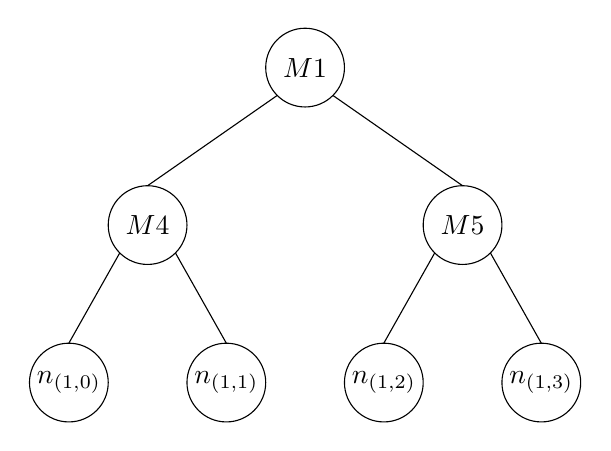
\begin{tikzpicture}[scale=0.5] % Adjust the scale factor as needed
        % Your TikZ code goes here
        \draw (0,0) circle (1cm);
        \node at (0,0) {$M1$};
        \draw (-4,-4) circle (1cm);
        \node at (-4,-4) {$M4$};
        \draw (4,-4) circle (1cm);
        \node at (4,-4) {$M5$};
        \draw (-6,-8) circle (1cm);
        \node at (-6,-8) {$n_{(1,0)}$};
        \draw (-2,-8) circle (1cm);
        \node at (-2,-8) {$n_{(1,1)}$};
        \draw (6,-8) circle (1cm);
        \node at (6,-8) {$n_{(1,3)}$};
        \draw (2,-8) circle (1cm);
        \node at (2,-8) {$n_{(1,2)}$};
        \draw ({0 + cos(225)},{0 + sin(225)}) -- (-4,-3);
        \draw ({0 + cos(315)},{0 + sin(315)}) -- (4,-3);
        \draw ({-4 + cos(225)},{-4 + sin(225)}) -- (-6,-7);
        \draw ({-4 + cos(315)},{-4 + sin(315)}) -- (-2,-7);
        \draw ({4 + cos(225)},{-4 + sin(225)}) -- (2,-7);
        \draw ({4 + cos(315)},{-4 + sin(315)}) -- (6,-7);
        


    \end{tikzpicture}
    \caption{Ways of Merging}
    \label{fig:ways_of_merging}
\end{figure}

\balance

\bibliographystyle{ACM-Reference-Format}
\bibliography{bibliography}

\end{document}
 

